% !TEX program = xelatex
\documentclass[11pt]{article}
\usepackage[margin=1in]{geometry}
\usepackage{amsmath, amssymb}
\usepackage{graphicx}
\usepackage{svg}
\usepackage{tikz-cd}
\usepackage{multicol}
\usepackage{tikz}
\usetikzlibrary{arrows.meta,positioning}
\newcommand*\circled[1]{\tikz[baseline=(char.base)]{
            \node[shape=circle,draw,inner sep=2pt] (char) {#1};}}
\usepackage{xcolor}
\usepackage[colorlinks=true,linkcolor=red,urlcolor=cyan,citecolor=blue]{hyperref}
\urlstyle{tt}

% Code
\usepackage{listings}
\lstset{
  basicstyle=\ttfamily\small,
  keywordstyle=\color{blue},
  commentstyle=\color{gray},
  stringstyle=\color{teal},
  columns=fullflexible,
  breaklines=true,
  backgroundcolor=\color{gray!15},
  frame=single,
  framerule=0pt,
  framesep=3pt,
  xleftmargin=5pt,
  xrightmargin=5pt
}

% Traditional Chinese support
\usepackage{fontspec}
\usepackage{xeCJK}
\setCJKmainfont{Noto Serif CJK TC}
\setCJKmonofont{Noto Serif CJK TC}

% Icon
\usepackage{fontawesome5}

\title{Robotic Navigation and Exploration\\HW2: Kinematic Models and Path Tracking Control\\Due Sunday, March 29, 2026 (11:59 PM)}
\author{}
\date{}

\begin{document}
\maketitle

\noindent\textbf{Student ID:} \underline{\makebox[5cm][l]{\textcolor{blue}{N26140692}}}\hfill\textbf{Name:} \underline{\makebox[5cm][l]{\textcolor{blue}{簡誌加}}} \\


\noindent To complete this assignment, make sure you have the following tools installed on your computer:
\begin{enumerate}
    \item Python version 3.8 +
    \item opencv-python
    \item numpy
    \item matplotlib
\end{enumerate}

\noindent Your written response must be typeset (\href{https://www.overleaf.com/read/xjnwwpbhzvhk#c13aac}{\LaTeX}) and in \textcolor{blue}{blue}. Also, do not forget to convert it into \textcolor{teal}{\texttt{report.pdf}} before submission.

\vspace{0.5em}
\noindent Please organize your submission into a folder as follows:
\vspace{0.5em}

\noindent
\fcolorbox{gray!15}{gray!15}{
    \begin{minipage}{\dimexpr\textwidth-2\fboxsep\relax}
        \vspace{0.5em}
        \hspace*{1em} \faFolderOpen\ \texttt{[your student ID]\_HW2/} \\
        \hspace*{2.5em} $\llcorner$ \faFilePdf\ \textcolor{teal}{\texttt{report.pdf}} \\
        \hspace*{2.5em} $\llcorner$ \faFolderOpen\ \texttt{code/} \\
        \hspace*{4.5em} $\llcorner$ $\cdots$
        \vspace{0.5em}
    \end{minipage}
}
\vspace{0.5em}

\noindent Then, compress this folder into a zip archive named \texttt{[your student ID]\_HW2.zip} and submit it to NTU COOL. \\
\textcolor{red}{\textbf{Warning:} A 10-point penalty will be applied if your submission does not follow this format.}

\section{Introduction}

This assignment focuses on the implementation and simulation of three fundamental \textbf{wheeled vehicle kinematic models}, alongside various \textbf{path-tracking control algorithms}. The primary objective is to enable an autonomous robot to robustly track a reference trajectory (generated in HW1) within a simulated environment.

The control architecture is decoupled into two parallel systems: \textbf{Longitudinal Control} and \textbf{Lateral Control}. First, you will build kinematic models for Basic, Differential Drive, and Bicycle configurations. Subsequently, longitudinal control algorithms will be implemented to generate safe velocity profiles and regulate the vehicle's speed along the track. Finally, you will develop multiple lateral tracking controllers—including PID, Pure Pursuit, Stanley, and LQR—to precisely minimize cross-track and heading errors. The assignment concludes by deploying these algorithms on simulated F1 circuits to evaluate their performance.
\begin{figure}[h]
    \centering
    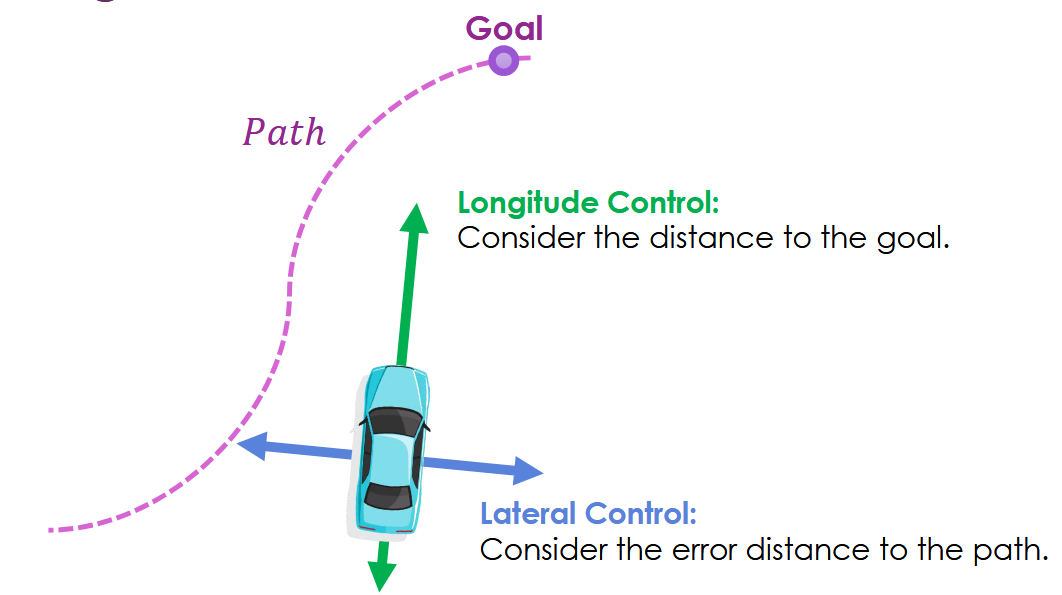
\includegraphics[width=0.6\linewidth]{image/longitude_lateral.png}
    \caption{Longitudinal Control and Lateral Control}
    \label{fig:longitude_lateral}
\end{figure}

\section{Kinematic Models}

To simulate realistic vehicle motion, this section formulates the state-update logic for three distinct kinematic models. Each mathematical model dictates how the vehicle's \textbf{state} $\boldsymbol{\zeta} = [x, y, \theta]^T$ evolves continuously subject to a given \textbf{control input} $\boldsymbol{u}$.

In the provided codebase, the \textcolor{teal}{\texttt{State}} object encapsulates not only the pose $(x, y, \theta)$ but also the vehicle's speed $v$ and angular velocity $\omega$. This formulation is particularly advantageous for models such as the bicycle model, where the direct control inputs are longitudinal acceleration $a$ and steering angle $\delta$; maintaining these dynamic states simplifies the discrete-time kinematic update. Note that throughout this document, $(x, y)$ denotes the 2D position, and $\theta$ represents the global heading (orientation).





\subsection{Basic Model}
\noindent The basic model assumes that the robot can be approximated as a single wheel rolling on a plane. It can move forward or rotate but cannot move sideways. \\

\begin{minipage}{0.3\textwidth}
    \centering
    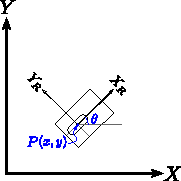
\includegraphics[width=\linewidth]{image/basic_model.pdf}
\end{minipage}
\hfill
\begin{minipage}{0.65\textwidth}
    \begin{itemize}
        \item Control State $\boldsymbol{u} = [v, \omega]^T$, where $v$ is the linear velocity and $\omega$ is the angular velocity.
        \item State: $\boldsymbol{\zeta} = [x, y, \theta]^T$, where $x, y$ is the position and $\theta$ is the orientation of the vehicle.
    \end{itemize}
    \begin{equation}
        \dot{\boldsymbol{\zeta}} =
        \begin{bmatrix}
            \dot{x} \\
            \dot{y} \\
            \dot{\theta}
        \end{bmatrix} = R(\theta)
        \begin{bmatrix}
            \dot{x_R} \\
            \dot{y_R} \\
            \dot{\theta}
        \end{bmatrix} =
        \begin{bmatrix}
            \cos\theta & -\sin\theta & 0 \\
            \sin\theta & \cos\theta  & 0 \\
            0          & 0           & 1
        \end{bmatrix}
        \begin{bmatrix}
            v \\
            0 \\
            \omega
        \end{bmatrix} =
        \begin{bmatrix}
            v \cos \theta \\
            v \sin \theta \\
            \omega
        \end{bmatrix}
    \end{equation}
\end{minipage}



\begin{enumerate}
    \item \noindent\textbf{\faPen} Check the code in \textcolor{teal}{\texttt{\detokenize{Simulation/}\allowbreak\detokenize{kinematic_basic.py}}}, and answer the following questions.
          \begin{enumerate}
              \item (2 pts) What is the unit of \texttt{yaw}? \\
                    \textcolor{blue}{degree}
              \item (2 pts) Why do we need \texttt{yaw = (state.yaw + state.w * self.dt) \% 360}? What would happen without this line? \\
                    \textcolor{blue}{We need this line to anticipate the yaw angle of the next moment, if we didn't have this line, we would not know the current direction the vehicle is facing}
          \end{enumerate}

    \item \noindent\textbf{\faPen}  (2 pts) In practice, a controller may output infeasible commands (e.g., exceeding the actuator limits).
          Therefore, our simulator applies constraints to the current state and/or control inputs.
          Please check the code in \textcolor{teal}{\texttt{\detokenize{Simulation/}\allowbreak\detokenize{simulator_basic.py}}} and list the constraints that are enforced.
          \begin{itemize}
            \color{blue}
                \item Linear Acceleration
                \item Linear Velocity
                \item Angular Velocity
          \end{itemize}
\end{enumerate}

\subsection{Differential Drive Model}
\noindent The differential drive model features two independently driven wheels on a shared axis. In this model, the control input becomes $[\dot{\phi}_{\mathrm{left}}, \dot{\phi}_{\mathrm{right}}]^T$, representing the angular velocities of the left and right wheels, respectively. \\

\begin{minipage}{0.3\textwidth}
    \centering
    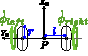
\includegraphics[width=\linewidth]{image/diff_drive_model2.pdf}
    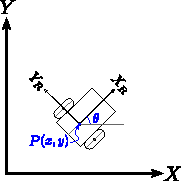
\includegraphics[width=\linewidth]{image/diff_drive_model.pdf}
\end{minipage}
\hfill
\begin{minipage}{0.7\textwidth}
    \begin{itemize}
        \item Control Input $\boldsymbol{u} = [\dot{\phi}_{\mathrm{left}}, \dot{\phi}_{\mathrm{right}}]^T$
        The control input can be mapped to $[v, \omega]$ by the following formula:
        \begin{align*}
            v      & = \frac{r}{2} (\dot{\phi}_{\mathrm{left}} + \dot{\phi}_{\mathrm{right}}) \\
            \omega & = \frac{r}{2l} (\dot{\phi}_{\mathrm{right}} - \dot{\phi}_{\mathrm{left}})
        \end{align*}
        \item State: $\boldsymbol{\zeta} = [x, y, \theta]^T$, where $x, y$ is the position and $\theta$ is the orientation of the vehicle.
    \end{itemize}
    \begin{equation}
        \dot{\boldsymbol{\zeta}} =
        \begin{bmatrix}
            \dot{x} \\
            \dot{y} \\
            \dot{\theta}
        \end{bmatrix} =
        \begin{bmatrix}
            v \cos \theta \\
            v \sin \theta \\
            \omega
        \end{bmatrix} =
        \begin{bmatrix}
            \frac{r}{2} (\dot{\phi}_{\mathrm{left}} + \dot{\phi}_{\mathrm{right}}) \cos \theta \\
            \frac{r}{2} (\dot{\phi}_{\mathrm{left}} + \dot{\phi}_{\mathrm{right}}) \sin \theta \\
            \frac{r}{2l} (\dot{\phi}_{\mathrm{right}} - \dot{\phi}_{\mathrm{left}})
        \end{bmatrix}
    \end{equation} \\
    \vspace{1.5em}
    \noindent
    \small
    \hspace*{1em} Related code in \textcolor{teal}{\texttt{\detokenize{Simulation/}\allowbreak\detokenize{kinematic_}\allowbreak\detokenize{differential_}\allowbreak\detokenize{drive.py}}}
\end{minipage} \\

For more details and derivations, please refer to the lecture slides (pp.24).
\begin{enumerate}
    \item \textbf{\faPen} (2 pts) Similar to 2.1.2, check the code in \textcolor{teal}{\texttt{\detokenize{Simulation/}\allowbreak\detokenize{simulator_differential_drive.py}}} and list the constraints that are enforced.
          \begin{itemize}
            \color{blue}
                \item Wheel Angular Acceleration
                \item Wheel Angular Velocity
          \end{itemize}
    \item \textbf{\faPython} (4 pts) Complete \textcolor{teal}{\texttt{\detokenize{# TODO 2.2.2}}} in \textcolor{teal}{\texttt{\detokenize{navigation.py}}}.
          For the following lateral control algorithm, the basic and differential drive models are implemented in the same file. However, for the differential drive model, you need to convert the control input $[v, \omega]$ into $[\dot{\phi}_{\mathrm{left}}, \dot{\phi}_{\mathrm{right}}]$.
          Run the command below to check the result of differential drive model:
          \begin{lstlisting}
$ python navigation.py -s diff_drive -c pid -t 400mRunningTrack
          \end{lstlisting}

          you should have similar result by running the following command:
          \begin{lstlisting}
$ python navigation.py -s basic -c pid -t 400mRunningTrack
          \end{lstlisting}

\end{enumerate}



\subsection{Bicycle Model}
\noindent The bicycle model is a simplified mathematical representation of a four-wheeled vehicle’s dynamics, reducing it to two wheels (one front, one rear) on a single track. \\

\begin{minipage}{0.3\textwidth}
    \centering
    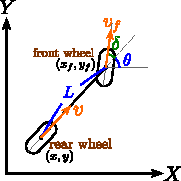
\includegraphics[width=\linewidth]{image/bicycle_model.pdf}
\end{minipage}
\hfill
\begin{minipage}{0.7\textwidth}
    \begin{itemize}
        \item Control Input $\boldsymbol{u} = [a, \delta]^T$, where $a$ is the linear acceleration and $\delta$ is the steering angle.
        \item State: $\boldsymbol{\zeta} = [x, y, \theta]^T$, where $x, y$ is the position and $\theta$ is the orientation of the vehicle.
    \end{itemize}
    \begin{equation}
        \dot{\boldsymbol{\zeta}} =
        \begin{bmatrix}
            \dot{x} \\
            \dot{y} \\
            \dot{\theta}
        \end{bmatrix} =
        \begin{bmatrix}
            v \cos \theta \\
            v \sin \theta \\
            \omega
        \end{bmatrix} =
        \begin{bmatrix}
            v \cos \theta \\
            v \sin \theta \\
            \frac{v}{L} \tan \delta
        \end{bmatrix}
    \end{equation}
    \begingroup
    \setlength{\leftskip}{1em}
    where $v$ is the velocity, $L$ is the wheelbase, and $\delta$ is the steering angle.
    \par\endgroup
\end{minipage} \\

For more details and derivations, please refer to the lecture slides (pp.32).
\begin{enumerate}
    \item \textbf{\faPython} (5 pts) According to the above formula, complete the \textcolor{teal}{\texttt{step()}} function in the \textcolor{teal}{\texttt{KinematicModelBicycle}} class which is defined in the file \textcolor{teal}{\path{Simulation/kinematic_bicycle.py}}
          \begin{lstlisting}
$ python navigation.py -s bicycle -c pid
          \end{lstlisting}
    \item \textbf{\faPen} (3 pts) Similar to 2.1.2, check the code in \textcolor{teal}{\texttt{\detokenize{Simulation/}\allowbreak\detokenize{simulator_bicycle.py}}} and list the constraints that are enforced.
          \begin{itemize}
            \color{blue}
                \item Linear Acceleration
                \item Steering Angle Rate
                \item Maximum Steering Angle
                \item Linear Velocity
          \end{itemize}
\end{enumerate}

\section{Path Tracking - Longitudinal Control}
In Homework 1, you generated the path geometry (waypoints). However, a raw path isn't enough for tracking; the vehicle needs a velocity profile to know when to slow down for corners and stay stable.

\begin{enumerate}
    \item \textbf{\faPython} Following the methodology below, complete the \textcolor{teal}{\texttt{generate\_speed\_profile()}} function in \textcolor{teal}{\texttt{\detokenize{trajectory_generator.py}}}

          Using these $(x, y)$ waypoints, compute a reference velocity profile $v_{\mathrm{ref}}$ for the entire trajectory. The velocity profile should be both \textbf{safe} (limited by curvature) and \textbf{dynamically feasible} (smooth acceleration/deceleration).

          \noindent\textbf{Algorithm outline:}
          \begin{enumerate}
              \item \textbf{Curvature $\kappa$:} Compute the curvature at each waypoint from the derivatives of the path coordinates. (already written)
              \item \textbf{Speed limit (4 pts):} Compute the maximum allowable speed based on lateral acceleration ($a_\mathrm{lat}=30\mathrm{m/s^2}$) and a global speed cap ($v_\mathrm{max}=85\mathrm{m/s}$):
                    \[
                        v_{\mathrm{limit}} = \min\left(v_{\max}, \sqrt{\frac{a_{\mathrm{lat}}}{\lvert\kappa\rvert}}\right).
                    \]
                    
                    \textbf{Hint:} In practice, $\kappa$ can be zero on straight segments. To avoid division by zero, add a small constant (e.g., $\epsilon = 10^{-6}$) to the denominator: $|\kappa| + \epsilon$.
              \item \textbf{Longitudinal smoothing (8 pts):} Apply a forward--backward pass ensuring the velocity profile respects acceleration and braking limits.
                    \begin{itemize}
                        \item \textbf{Forward pass:} limit acceleration ($a_{\mathrm{acc}}=12\mathrm{m/s^2}$).
                              \[
                                  v_i^2 \le v_{i-1}^2 + 2\cdot a_{\mathrm{acc}} \cdot ds
                              \]
                        \item \textbf{Backward pass:} limit deceleration ($a_{\mathrm{dec}}=18\mathrm{m/s^2}$) so the vehicle slows down before corners.
                              \[
                                  v_i^2 \le v_{i+1}^2 + 2\cdot a_{\mathrm{dec}} \cdot ds
                              \]
                        \item \textbf{Launch Restrictions:}
                              \begin{itemize}
                                  \item Starting Speed ($v_{\mathrm{ref}}[0]$): 5.0 m/s
                                  \item Terminal Target Speed ($v_{\mathrm{ref}}[-1]$): 0.0 m/s
                              \end{itemize}
                    \end{itemize}
                    \textbf{Hint:} Think carefully about where to apply each restriction.
          \end{enumerate}
          Run the following command to check your velocity profile:
          \begin{lstlisting}
$ python trajectory_generator.py
          \end{lstlisting}

    \item \textbf{\faPython} (8 pts) \textbf{Speed Tracking with PID:} In our bicycle model, the longitudinal control input is the vehicle's acceleration $a$. Please implement a PID controller that calculates the appropriate acceleration to effectively track the reference speed $v_{\mathrm{ref}}$. 
          The default gains $K_p$, $K_i$, and $K_d$ are already provided in the code, but feel free to fine-tune them!


          \noindent\textbf{PID formula:}
          \[
              e(t) = v_{\mathrm{ref}}(t) - v(t),
              \qquad
              u(t) = a = K_p\,e(t) + K_i\int_0^t e(\tau)\,d\tau + K_d\,\frac{de(t)}{dt}.
          \]

          Run the following command to check your longitudinal PID controller:
          \begin{lstlisting}
$ python navigation.py -s bicycle -c pid -t 1000mStraight
          \end{lstlisting}
\end{enumerate}



\section{Path Tracking - Lateral Control}

\subsection{PID Control}

PID control works just as well for lateral tracking. The main difference is simply how we define the tracking error.

\begin{enumerate}
    \item \textbf{\faPen} (2 pts) According to \textcolor{teal}{\texttt{\detokenize{PathTracking/}\allowbreak\detokenize{controller_pid_basic.py}}}, identify the error term of PID lateral control. \\
            \begin{minipage}{\linewidth}
                \centering
                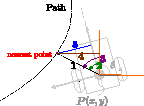
\includegraphics[width=0.5\linewidth]{image/PID_Lateral.pdf}
            \end{minipage}
            \textcolor{blue}{1.min\_dist 2.theta\_err 3.theta\_target 4.target[0]-x 5.err}
    \item \textbf{\faPython}\textbf{\faPen} (5 pts) Tune the PID gains $K_p$, $K_i$, and $K_d$ in \textcolor{teal}{\texttt{\detokenize{PathTracking/}}}\allowbreak\textcolor{teal}{\texttt{\detokenize{controller_pid_basic.py}}} to achieve the best performance,
          and briefly describe how you tuned the PID gains $K_p$, $K_i$, and $K_d$. It is recommended to include a screenshot of the resulting trajectory. \\
          \textbf{Hint:} You may refer to \href{https://tlk-energy.de/blog-en/practical-pid-tuning-guide}{PID Tuning Guide} (or any other PID-tuning method).
          \begin{lstlisting}
$ python navigation.py -s basic -c pid -t 1000mStraight --init_shift 1.5
          \end{lstlisting}
          \textcolor{blue}{Initially, the PID lateral controller used kp=0.1, ki=0.005, and kd=0.015. At a high speed of 85 m/s, this caused severe steering oscillation and a large average cross-track error of 1.71 meters. Analysis revealed that the integral term accumulated unnecessary error, leading to overshoot, while the derivative term was too weak to dampen the steering velocity. The tuning strategy focused on eliminating the integral term to prevent windup and significantly increasing the derivative term to act as a strong damper. By applying the final parameters of kp=0.1, ki=0.0, and kd=0.5, the vehicle stabilized, successfully reducing the average error to 0.38 meters.} \\
          \begin{minipage}{\linewidth}
            \centering
            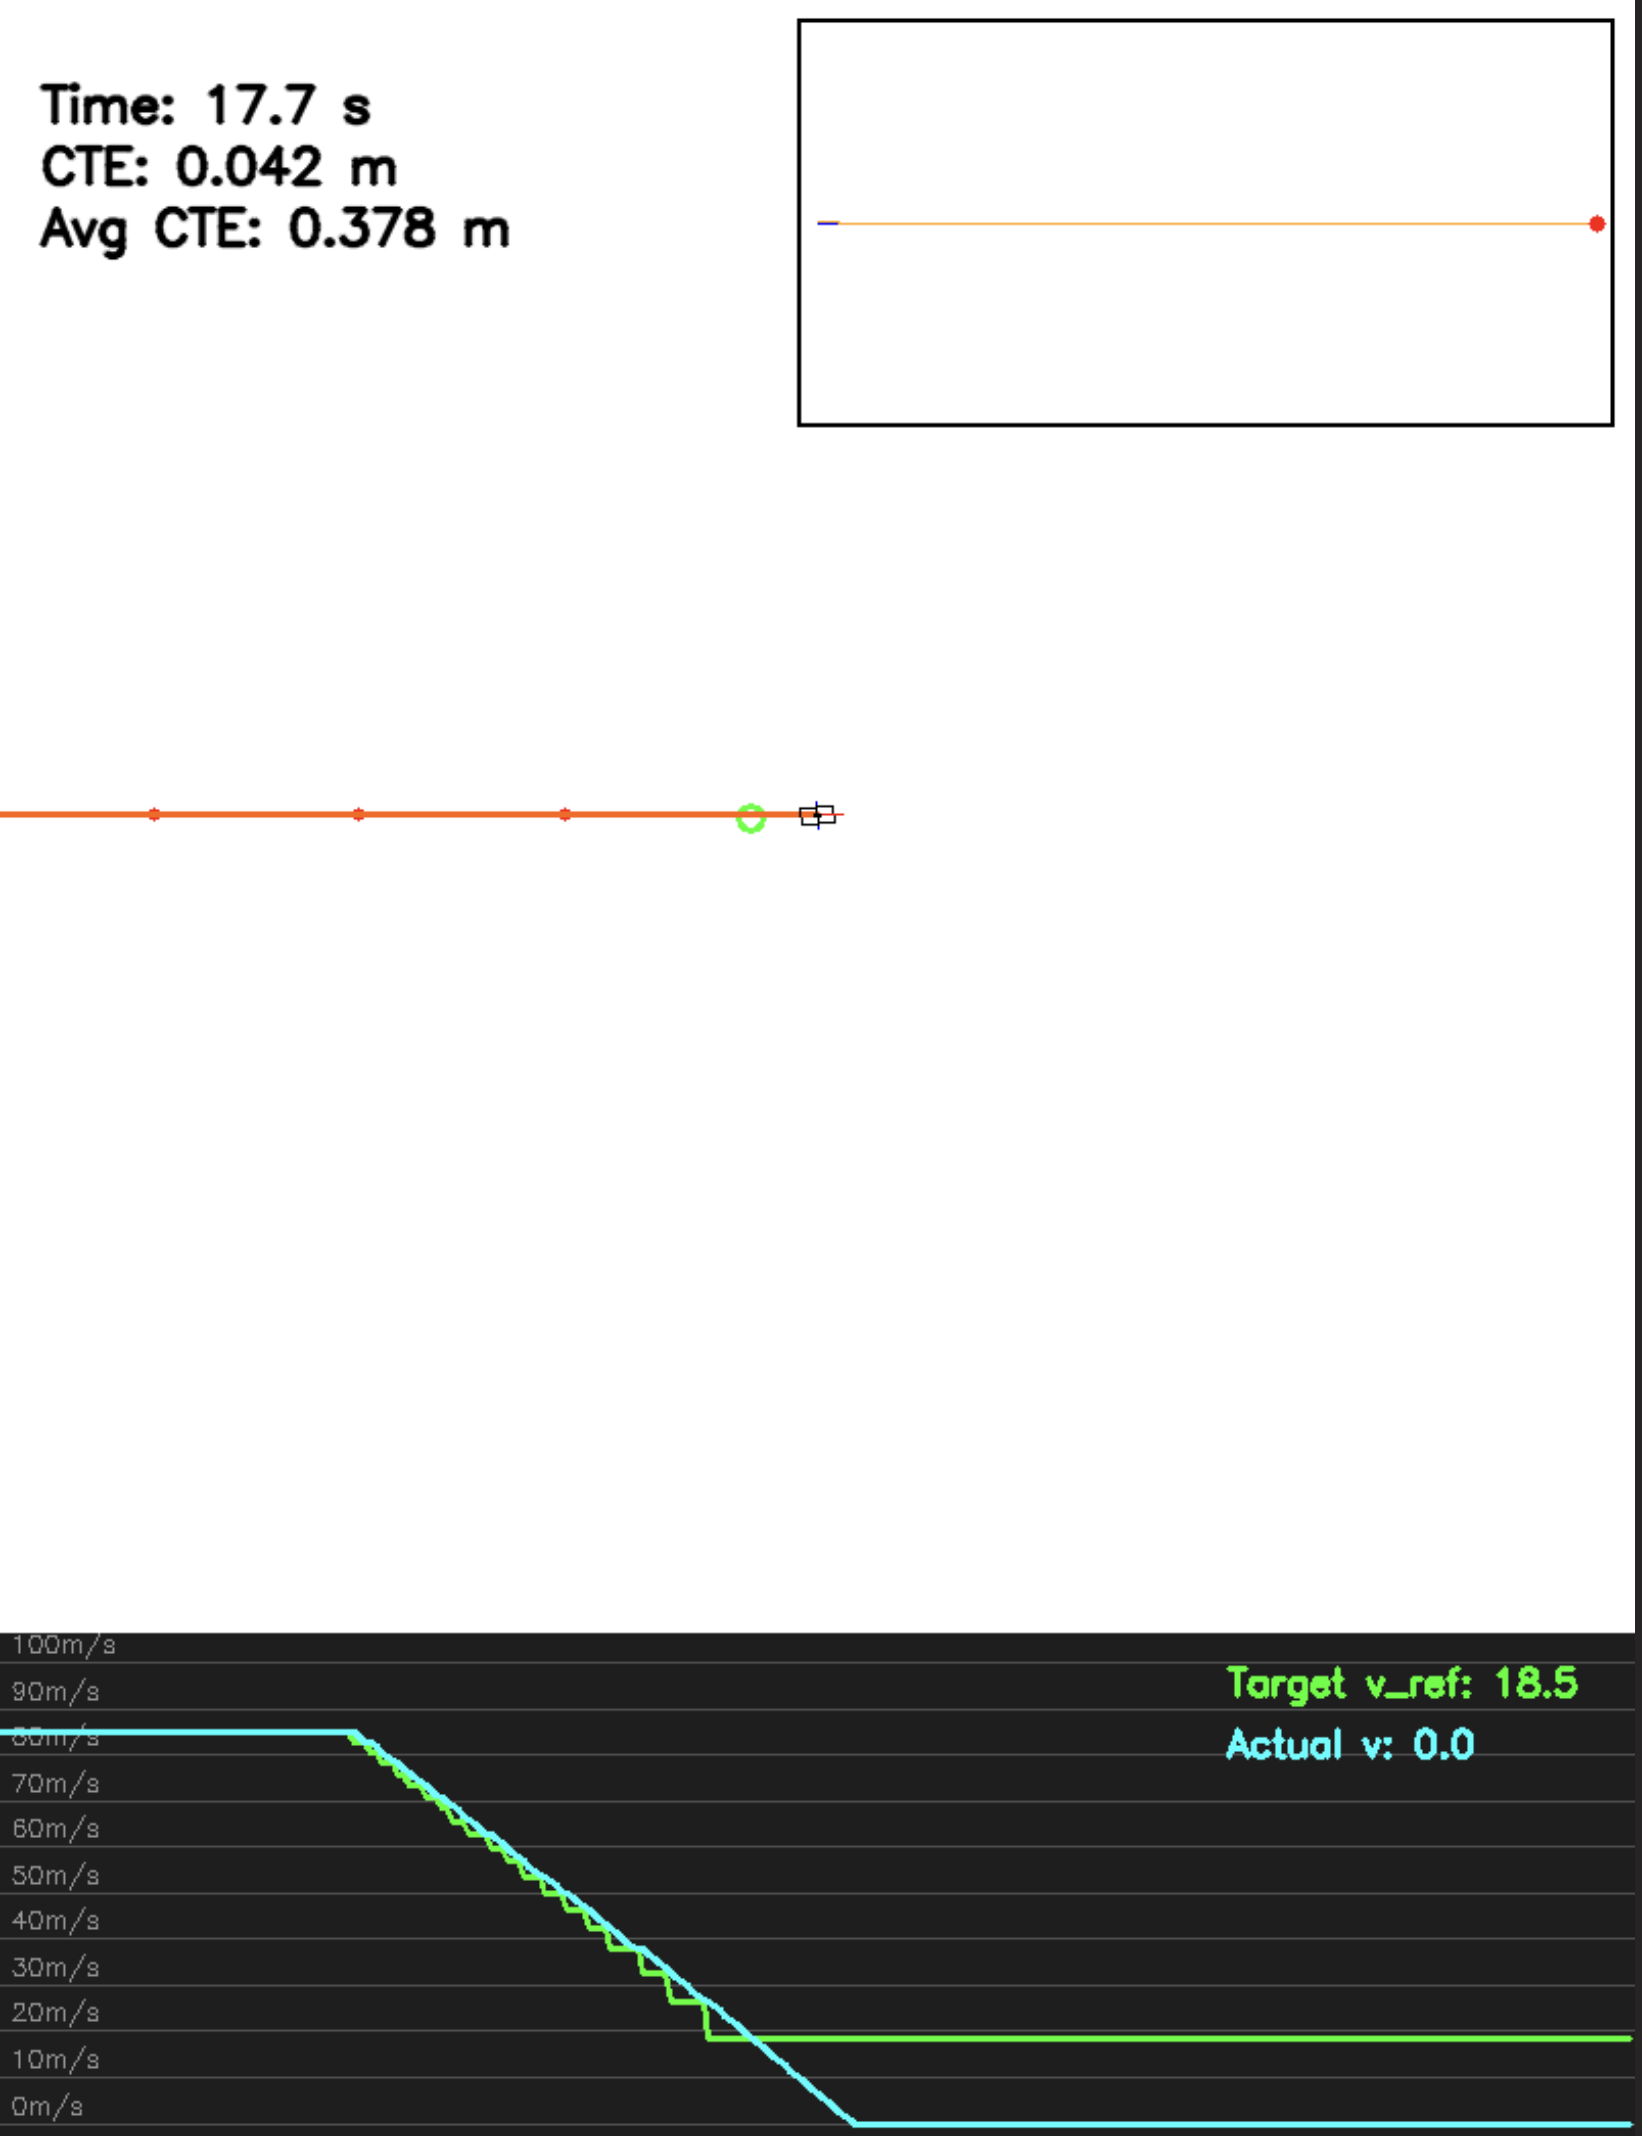
\includegraphics[width=0.43\linewidth]{image/4.1.2.png}
        \end{minipage}

    \item \textbf{\faPython}\textbf{\faPen} (5 pts) For the bicycle model, you may choose whether to use the same error definition as the basic model. If not, please describe the error you used. Complete \textcolor{teal}{\texttt{\detokenize{PathTracking/}}}\allowbreak\textcolor{teal}{\texttt{\detokenize{controller_pid_bicycle.py}}} \\
          Run the following command to check your PID controller:
          \begin{lstlisting}
$ python navigation.py -s bicycle -c pid -t 400mRunningTrack
          \end{lstlisting}

          \textcolor{blue}{your answer (if you changed the error definition)}
\end{enumerate}


\subsection{Pure Pursuit Control}

The Pure Pursuit algorithm calculates the steering angle $\delta$ needed to guide the vehicle toward a "look-ahead" point on the path. \\

\begin{minipage}{0.5\linewidth}
    \centering
    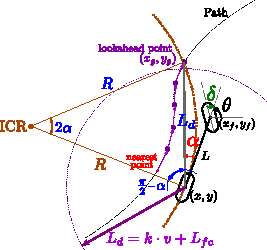
\includegraphics[width=\linewidth]{image/pure_pursuit.pdf}
\end{minipage}
\hfill
\begin{minipage}{0.45\linewidth}
    \textbf{Pure Pursuit Algorithm}
    \begin{enumerate}
        \item Find the nearest point on the path.
        \item Find the first point on the path that is at least $L_d$ away.
              \begin{equation*}
                  L_d = k \times v + L_{fc}
              \end{equation*}
        \item Calculate the steering angle $\delta$ to move the vehicle toward the "look-ahead" point.
              \begin{equation*}
                  \delta = \arctan\left(\frac{2L\sin(\alpha)}{L_d}\right)
              \end{equation*}
    \end{enumerate}
\end{minipage} \\

For more details and derivations, please refer to the lecture slides (pp.~34).
\begin{enumerate}
    \item \textbf{\faPython} (8 pts) According to the above algorithm, complete \textcolor{teal}{\path{PathTracking/controller_pure_pursuit_bicycle.py}}
    \begin{lstlisting}
$ python navigation.py -s bicycle -c pure_pursuit -t 400mRunningTrack
    \end{lstlisting}
\end{enumerate}


\subsection{Stanley Control}

Stanley control is a path-tracking algorithm that determines the steering angle by combining the \textbf{heading error} relative to the path with the \textbf{cross-track error} measured from the center of the front axle to the nearest point on the path. \\

\begin{minipage}{0.4\linewidth}
    \centering
    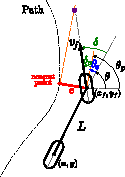
\includegraphics[width=\linewidth]{image/stanley.pdf}
\end{minipage}
\hfill
\begin{minipage}{0.5\linewidth}
    \textbf{Stanley Control Algorithm}
    \begin{enumerate}
        \item Find the nearest point on the path.
        \item Calculate the heading error $\theta_e$ and the cross-track error $\delta_e$.
              \begin{equation*}
                  \theta_e = \theta_{path} - \theta
              \end{equation*}
              \begin{equation*}
                  |e| = \sqrt{(x - x_{path})^2 + (y - y_{path})^2}
              \end{equation*}
        \item Calculate the steering angle $\delta$ to move the vehicle toward the "look-ahead" point.
              \begin{equation}\label{eq:stanley}
                  \delta = \theta_e + \delta_e = \theta_e + \arctan\left(\frac{-ke}{v_f}\right)
              \end{equation}
    \end{enumerate}
\end{minipage} \\

For more details and derivations, please refer to the lecture slides (pp.~35).

\begin{enumerate}
    \item \textbf{\faPython} (8 pts) According to the above algorithm, complete \textcolor{teal}{\path{PathTracking/controller_stanley_bicycle.py}}
    \begin{lstlisting}
$ python navigation.py -s bicycle -c stanley -t 400mRunningTrack
    \end{lstlisting}
    \textbf{Hint1:} Pay attention to the magnitude of $\theta_e$ \\
    \textbf{Hint2:} Be careful about the sign of $e$, where $\dot{e} = v_f\sin(\delta_e)$ in deviation of Eq.~(\ref{eq:stanley}).
\end{enumerate}



\subsection{LQR Control}

\subsubsection*{Problem Formulation}

Given a discrete-time linear system:
\begin{equation}
    \mathbf{x}_{k+1} = A \mathbf{x}_k + B \mathbf{u}_k
\end{equation}

The goal of LQR is to find an optimal control sequence $\mathbf{u}_k$ that minimizes the overall cost function $J$:
\begin{equation}
    J = \sum_{k=0}^{\infty} (\mathbf{x}_k^T Q \mathbf{x}_k + \mathbf{u}_k^T R \mathbf{u}_k)
\end{equation}

\begin{itemize}
    \item $Q$ (State Weight Matrix): Penalizes deviations from the desired state (error).
    \item $R$ (Control Weight Matrix): Penalizes the control effort (energy expenditure).
\end{itemize}

\subsubsection*{The Matrix P (Cost-to-Go)}

The matrix $P$ is the key to solving LQR and represents the ``Cost-to-Go''.

\begin{itemize}
    \item \textbf{Value Function $V(\mathbf{x})$:}
          The value function $V(\mathbf{x}_k)$ tells us the minimum cost from our current state $\mathbf{x}_k$ all the way to infinity:
          \begin{equation}
              V(\mathbf{x}_k) = \min_{\mathbf{u}_k, \mathbf{u}_{k+1}, \dots} \sum_{i=k}^{\infty} \left( \mathbf{x}_i^T Q \mathbf{x}_i + \mathbf{u}_i^T R \mathbf{u}_i \right)
          \end{equation}
          For LQR, this value function is quadratic and is defined by the matrix $P$:
          \begin{equation}
              V(\mathbf{x}_k) = \mathbf{x}_k^T P \mathbf{x}_k
          \end{equation}
          Then, we can write the recursive form of value function:
          \begin{equation}
              \begin{split}
                  V(\mathbf{x}_k) &= \min_{\mathbf{u}} \{ \mathbf{x}_k^T Q \mathbf{x}_k + \mathbf{u}_k^T R \mathbf{u}_k +V(x_{k+1})\} \\
                  &= \min_{\mathbf{u}} \{ \mathbf{x}_k^T Q \mathbf{x}_k + \mathbf{u}_k^T R \mathbf{u}_k +\mathbf{x}^T_{k+1}P\mathbf{x}_{k+1}\}
              \end{split}
          \end{equation}
    \item \textbf{Significance:}
          \begin{itemize}
              \item $P$ condenses the entire future trajectory dynamics and costs into a single matrix.
              \item It measures the total future cost starting from state $\mathbf{x}_k$.
          \end{itemize}
\end{itemize}

To find $P$, we must solve the Discrete Algebraic Riccati Equation (DARE):
\begin{equation}
    P = A^T P A - (A^T P B)(R + B^T P B)^{-1} (B^T P A) + Q
\end{equation}
The related code can be found in the function \textcolor{teal}{\texttt{\detokenize{_solve_DARE()}}} in \textcolor{teal}{\texttt{\detokenize{PathTracking/}\allowbreak\detokenize{controller_lqr_bicycle.py}}}.

\subsubsection*{The Optimal Control Law}

Once $P$ is obtained, the optimal control input $\mathbf{u}_k$ is a linear state feedback law:
\begin{equation}
    \mathbf{u}_k = -K \mathbf{x}_k
\end{equation}

Where $K$ is the optimal gain matrix derived from $P$:
\begin{equation}
    K = (R + B^T P B)^{-1} (B^T P A)
\end{equation}

The derivation process of $K$ is detailed in lecture slides (pp.39).


\begin{enumerate}
    \item \textbf{\faPython} (8 pts) We assume the state is $\mathbf{x} = [e, \theta_e]^T$, where $e$ is the cross-track error and $\theta_e$ is the heading error,
          and the control input is $\mathbf{u} = [\delta]^T$.
          For the bicycle model, we have the following kinematic equations: \\
          \begin{minipage}{0.4\linewidth}
            \centering
            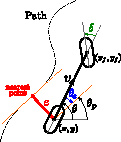
\includegraphics[width=\linewidth]{image/LQR.pdf}
          \end{minipage}
          \hfill
          \begin{minipage}{0.55\linewidth}
            \begin{equation*}
                \dot{e} = -v \sin(\theta_e)
            \end{equation*}
            \begin{equation*}
                \dot{\theta}_e = -\frac{v}{L} \tan(\delta)
            \end{equation*}
            In LQR, we assume that $\theta_e$ and $\delta$ are small, so we can approximate $\sin(\theta_e) \approx \theta_e$ and $\tan(\delta) \approx \delta$,
            then we have
            \begin{equation}\label{eq:lqr_e}
                \dot{e} = -v \theta_e
            \end{equation}
            \begin{equation}\label{eq:lqr_thetae}
                \dot{\theta}_e = -\frac{v}{L} \delta
            \end{equation}
            and
            \begin{equation*}
                \begin{bmatrix} \dot{e} \\ \dot{\theta}_e \end{bmatrix} =
                \begin{bmatrix} 0 & -v \\ 0 & 0 \end{bmatrix}
                \begin{bmatrix} e \\ \theta_e \end{bmatrix} + \begin{bmatrix} 0 \\ -\frac{v}{L} \end{bmatrix} \delta
            \end{equation*}
          \end{minipage}
          Then the linear system would be:
          \begin{equation*}
              \begin{split}
                  \mathbf{x}_{k+1} & = A \mathbf{x}_k + B \mathbf{u}_k                                                                                            \\
                                   & = \begin{bmatrix} e_k \\ \theta_{e,k} \end{bmatrix} + \begin{bmatrix} \dot{e_k} \\ \dot{\theta}_{e,k} \end{bmatrix} \Delta t \\
                                   & = \begin{bmatrix} 1 & -v\cdot \Delta t \\ 0 & 1 \end{bmatrix}
                  \begin{bmatrix} e_k \\ \theta_{e,k} \end{bmatrix} +
                  \begin{bmatrix} 0 \\ -\frac{v}{L} \Delta t \end{bmatrix}
                  \begin{bmatrix} \delta_k \end{bmatrix}
              \end{split}
          \end{equation*}
          Please refer to the equations above and complete the code in \textcolor{teal}{\path{PathTracking/controller_lqr_bicycle.py}}
          \begin{lstlisting}
$ python navigation.py -s bicycle -c lqr -t 400mRunningTrack --lqr_control_state steering_angle
          \end{lstlisting}
          \textbf{Hint1:} Pay attention to the magnitude of $\theta_e$ \\
          \textbf{Hint2:} Ensure that the definitions of $\theta_e$, $e$, and $\delta$ in your code are consistent with Eq.~(\ref{eq:lqr_e}) and~(\ref{eq:lqr_thetae}).
    \item \textbf{\faPen} (4 pts) Write down how you choose the weight matrices $Q$ and $R$ \\
          \textcolor{blue}{To determine the weight matrices Q and R for the steering\_angle control state, I conducted a series of iterative trials. Initially, I used default identity matrices (Q11=1, Q22=1, R11=1). Since pure LQR struggles with steady-state error during curves, the vehicle severely understeered at high speeds, lost the track, and flew off. Next, I tried highly aggressive weights (Q11=500, Q22=50, R11=0.1) to force the car onto the path. While it successfully finished the lap, it caused severe high-frequency steering chattering due to over-sensitivity. After introducing feedforward control to handle the curve's baseline steering angle, I tested a balanced setup (Q11=10, Q22=1, R11=1). This achieved an incredibly low average cross-track error of 0.022 meters, but minor steering jitter remained. Ultimately, to prioritize ride smoothness and actuator lifespan over microscopic tracking precision, I selected the final parameters: Q11=10, Q22=1, and R11=10. By maintaining a strong penalty on cross-track error (Q11=10) but significantly increasing the penalty on steering effort (R11=10), the high-frequency control oscillations were successfully suppressed. This provided a much smoother and physically realistic steering response, with only a negligible increase in average error to 0.0244 meters.}
    \item \textbf{\faPen} (4 pts) Now, to regulate the steering speed, we need to change the control input $\mathbf{u}$ to the steering angular velocity, $\dot{\delta}$.
          The state then becomes $\mathbf{x} = [e, \theta_e, \delta]^T$. \\
          Please finish the linear system below:
          \begin{equation*}
              \begin{split}
                  \mathbf{x}_{k+1} & = A \mathbf{x}_k + B \mathbf{u}_k                                                                                                                                                                                                                                                                                                        \\
                                   & = \begin{bmatrix} e_k \\ \theta_{e,k} \\ \delta_k \end{bmatrix} + \begin{bmatrix} \dot{e_k} \\ \dot{\theta}_{e,k} \\ \dot{\delta}_k \end{bmatrix} \Delta t                                                                                                                                                                               \\
                                   & = \begin{bmatrix} 
                                    \textcolor{blue}{1} & \textcolor{blue}{v \Delta t} & \textcolor{blue}{0} \\ 
                                    \textcolor{blue}{0} & \textcolor{blue}{1} & \textcolor{blue}{\frac{v \Delta t}{L}} \\ 
                                    \textcolor{blue}{0} & \textcolor{blue}{0} & \textcolor{blue}{1} \end{bmatrix}
                  \begin{bmatrix} e_k \\ \theta_{e,k} \\ \delta_k \end{bmatrix} +
                  \begin{bmatrix} 
                    \textcolor{blue}{0} \\ 
                    \textcolor{blue}{0} \\ 
                    \textcolor{blue}{\Delta t} \end{bmatrix}
                  \begin{bmatrix} \dot{\delta}_k \end{bmatrix}
              \end{split}
          \end{equation*}
    \item \textbf{\faPython} (6 pts) Based on the previous question, complete \textcolor{teal}{\texttt{\detokenize{PathTracking/}\allowbreak\detokenize{controller_lqr_bicycle.py}}}
          \begin{lstlisting}
$ python navigation.py -s bicycle -c lqr -t 400mRunningTrack --lqr_control_state steering_angular_velocity
          \end{lstlisting}
\end{enumerate}

\section{F1 Track Challenge}
\begin{enumerate}
    \item \textbf{\faPython} (10 pts) Now that you've built these models and controllers, it's time to put them to the test on some actual F1 circuits! 
          We provide three F1 circuits: Silverstone, Suzuka, and Monza. You are free to choose whichever combination of kinematic model (basic, differential drive, or bicycle) and controller (PID, Pure Pursuit, Stanley, or LQR) that yields the best performance on average across all three tracks.
          You can tune controller parameters, implement additional controllers, or improve any part of the navigation flow to enhance overall system performance.

          \begin{lstlisting}[backgroundcolor=\color{gray!15}, frame=single, framerule=0pt, framesep=5pt, xleftmargin=5pt, xrightmargin=5pt]
$ python navigation.py -s [basic|diff_drive|bicycle] -c [pid|pure_pursuit|stanley|lqr] -t [Silverstone|Suzuka|Monza]
          \end{lstlisting}
          \textbf{Rules: }
          \begin{itemize}
            \item Do not change the constraints $v_\mathrm{max}$, $a_\mathrm{lat}$, $a_\mathrm{acc}$, $a_\mathrm{dec}$ in velocity profiling or any simulator code.
            \item If you modify any code outside the designated \texttt{\#TODO} blocks, please mark them with a \texttt{\#NewFeature} comment and describe the changes in your report.
            \item \textcolor{red}{Any violation of the above rules will receive 0 points in this challenge!}
          \end{itemize}



          \textbf{Grading Policy:} 
          Let $T_{\mathrm{ref},i}$ be the baseline completion time for track $i$ (\textbf{Silverstone: 107s, Suzuka: 115s, Monza: 94s}).
          \begin{align*}
              S_{T,i} &= \max \left( 0,\; \min \left( 6,\; 4 - k_T (T_i - T_{\mathrm{ref},i}) \right) \right) \\
              S_{E,i} &= \max \left( 0,\; \min \left( 6,\; 4 - k_E (E_i - 1.5) \right) \right) \\
              \text{Score}_i &= \min \left( 10,\; S_{T,i} + S_{E,i} \right) \\
              \text{Final Score} &= \left\lceil \frac{1}{3} \sum_{i} \text{Score}_i \right\rceil
          \end{align*}
          Here, $k_T = 0.5$ and $k_E = 2.0$ are penalty coefficients. Note that tracking error is penalized more heavily than completion time, so prioritize accuracy over speed. Try your best!
          
          \textbf{\faPen} Write down your command for this challenge, and put the screenshot of your result.
          \begin{lstlisting}[backgroundcolor=\color{gray!15}, frame=single, framerule=0pt, framesep=5pt, xleftmargin=5pt, xrightmargin=5pt, escapeinside={(*@}{@*)}]
$ python navigation.py -s (*@\textcolor{blue}{your\_model}@*) -c (*@\textcolor{blue}{your\_controller}@*) -t [Silverstone|Suzuka|Monza]
          \end{lstlisting}
        \begin{minipage}{\linewidth}
            \centering
            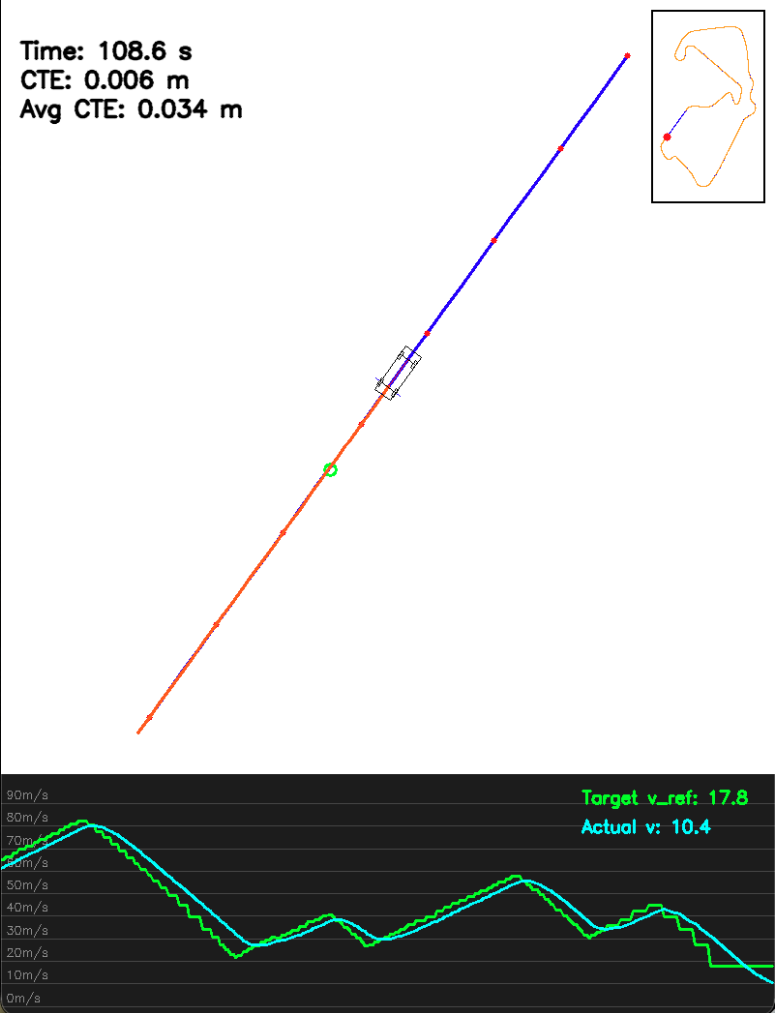
\includegraphics[width=0.43\linewidth]{image/Silverstone.png}
        \end{minipage}
        \begin{lstlisting}[backgroundcolor=\color{gray!15}, frame=single, framerule=0pt, framesep=5pt, xleftmargin=5pt, xrightmargin=5pt, escapeinside={(*@}{@*)}]
$ python navigation.py -s (*@\textcolor{blue}{bicycle}@*) -c (*@\textcolor{blue}{lqr}@*) -t (*@\textcolor{blue}{Silverstone}@*) --lqr_control_state (*@\textcolor{blue}{steering\_angle}@*)
          \end{lstlisting}
        \begin{minipage}{\linewidth}
            \centering
            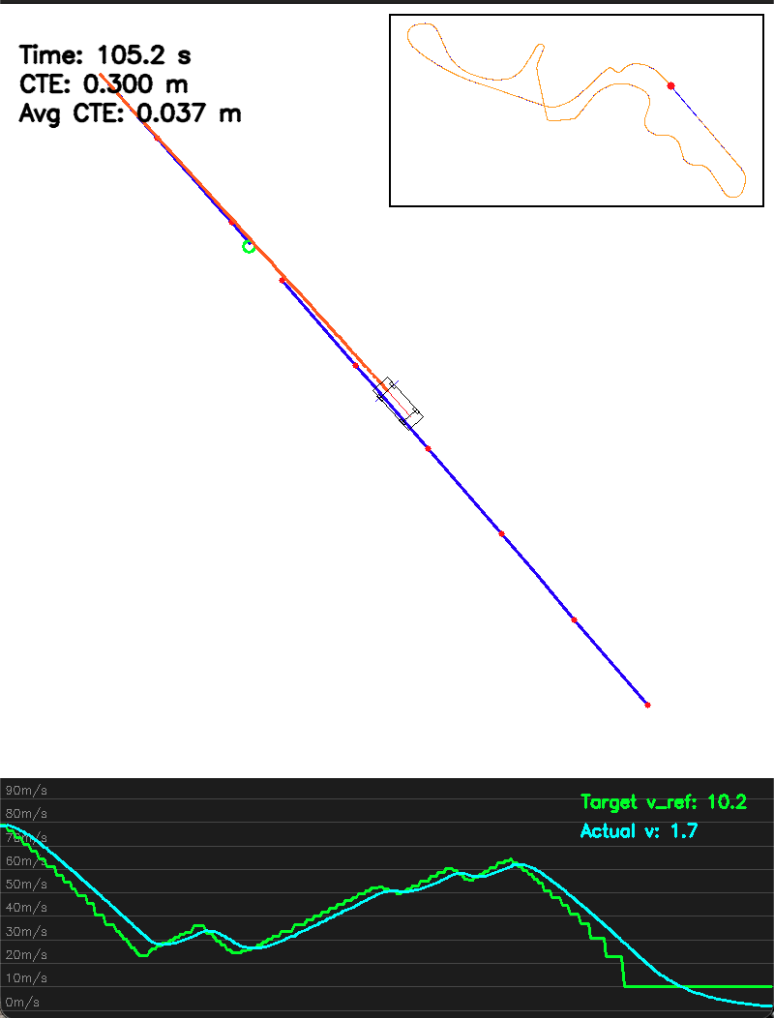
\includegraphics[width=0.43\linewidth]{image/Suzuka.png}
        \end{minipage}
        \begin{lstlisting}[backgroundcolor=\color{gray!15}, frame=single, framerule=0pt, framesep=5pt, xleftmargin=5pt, xrightmargin=5pt, escapeinside={(*@}{@*)}]
$ python navigation.py -s (*@\textcolor{blue}{bicycle}@*) -c (*@\textcolor{blue}{lqr}@*) -t (*@\textcolor{blue}{Suzuka}@*) --lqr_control_state (*@\textcolor{blue}{steering\_angle}@*)
          \end{lstlisting}
        \begin{minipage}{\linewidth}
            \centering
            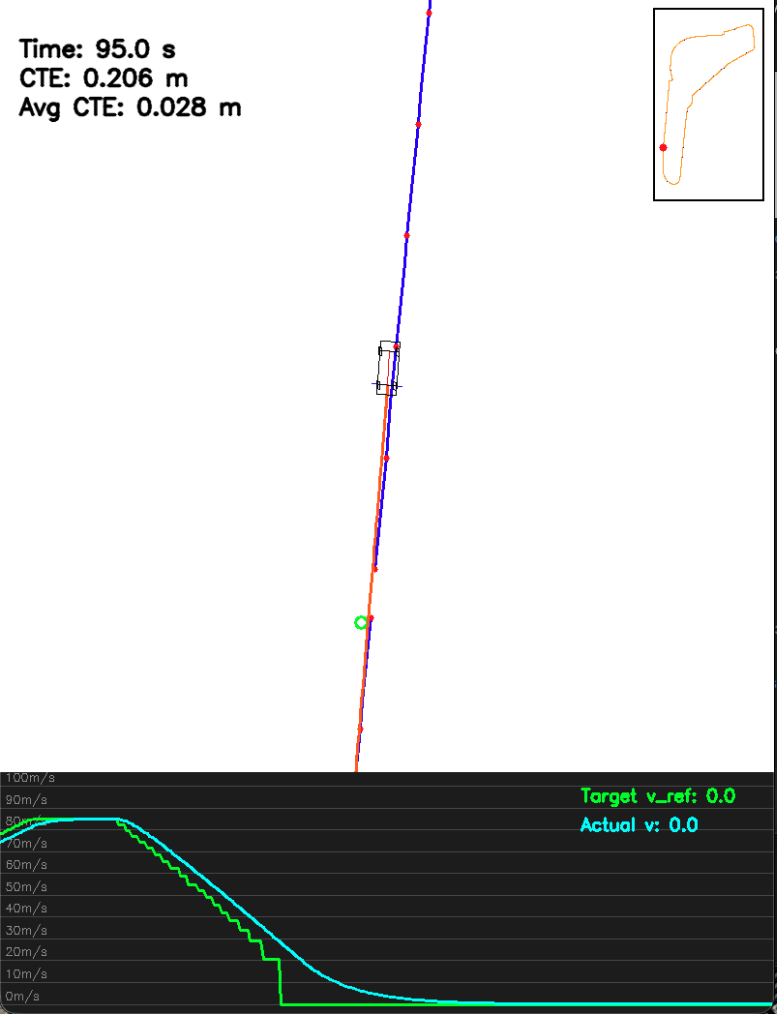
\includegraphics[width=0.43\linewidth]{image/Monza.png}
        \end{minipage}
        \begin{lstlisting}[backgroundcolor=\color{gray!15}, frame=single, framerule=0pt, framesep=5pt, xleftmargin=5pt, xrightmargin=5pt, escapeinside={(*@}{@*)}]
$ python navigation.py -s (*@\textcolor{blue}{bicycle}@*) -c (*@\textcolor{blue}{lqr}@*) -t (*@\textcolor{blue}{Monza}@*) --lqr_control_state (*@\textcolor{blue}{steering\_angle}@*)
          \end{lstlisting}
    \item \textbf{\faPen} (Extra up to +5 pts) Describe what you have tried to improve the performance: \\
          \textcolor{blue}{Your answer}
        \end{enumerate}

\section{Feedback (Optional)}
\begin{enumerate}
    \item \textbf{\faPen} (Extra up to +5 pts) We would love to hear your feedback on this homework! Please write down your thoughts, any difficulties you encountered, or suggestions for improving this assignment. 
          Your feedback will be highly valuable for future improvements. \\
          \textcolor{blue}{Your feedback}
\end{enumerate}


\clearpage
\section*{Assignment Checklist}

\noindent Please check the boxes ($\square \rightarrow \blacksquare$) which you have completed

\begin{table}[h!]
    \centering
    \begin{tabular}{|c|c|c|p{11cm}|c|}
        \hline
        \textbf{Done}                              & \textbf{No.} & \textbf{Type}    & \textbf{Task}                                                                                    & \textbf{Points} \\ \hline
        $\blacksquare$                                  & 2.1.1        & \faPen           & Answer questions (yaw unit, update) about \texttt{kinematic\_basic.py}                           & 4               \\ \hline
        $\blacksquare$                                  & 2.1.2        & \faPen           & List constraints about \texttt{simulator\_basic.py}                                              & 2               \\ \hline
        $\blacksquare$                                  & 2.2.1        & \faPen           & List constraints regarding \texttt{simulator\_different\_drive.py}                               & 2               \\ \hline
        $\blacksquare$                                  & 2.2.2        & \faPython        & Complete \# TODO 2.2.2 in \texttt{navigation.py} for differential drive                          & 4               \\ \hline
        $\blacksquare$                                  & 2.3.1        & \faPython        & Complete \texttt{step()} in \texttt{KinematicModelBicycle}                                       & 5               \\ \hline
        $\blacksquare$                                  & 2.3.2        & \faPen           & List constraints regarding \texttt{simulator\_bicycle.py}                                        & 3               \\ \hline
        $\blacksquare$                                  & 3.1          & \faPython        & Complete velocity profiling in \texttt{trajectory\_generator.py} (Speed limit 4 pts + Smoothing 8 pts) & 12              \\ \hline
        $\blacksquare$                                  & 3.2          & \faPython        & Implement Longitudinal PID control in \texttt{navigation.py}                                     & 8               \\ \hline
        $\blacksquare$                                  & 4.1.1        & \faPen           & Identify error term in \texttt{PathTracking/controller\_pid\_basic.py}                           & 2               \\ \hline
        $\blacksquare$                                  & 4.1.2        & \faPython/\faPen & Tune PID gains in \texttt{controller\_pid\_basic.py} and describe tuning process                 & 5               \\ \hline
        $\blacksquare$                                  & 4.1.3        & \faPython/\faPen & Complete \texttt{PathTracking/controller\_pid\_bicycle.py}                                       & 5               \\ \hline
        $\blacksquare$                                  & 4.2.1        & \faPython        & Complete \texttt{PathTracking/controller\_pure\_pursuit\_bicycle.py}                             & 8               \\ \hline
        $\blacksquare$                                  & 4.3.1        & \faPython        & Complete \texttt{PathTracking/controller\_stanley\_bicycle.py}                                   & 8               \\ \hline
        $\blacksquare$                                  & 4.4.1        & \faPython        & Complete \texttt{PathTracking/controller\_lqr\_bicycle.py}                                       & 8               \\ \hline
        $\blacksquare$                                  & 4.4.2        & \faPen           & Write down how you choose the weight matrices $Q$ and $R$                                        & 4               \\ \hline
        $\blacksquare$                                  & 4.4.3        & \faPen           & Complete linear system of Equation (19)                                                          & 4               \\ \hline
        $\blacksquare$                                  & 4.4.4        & \faPython        & Complete \texttt{PathTracking/controller\_lqr\_bicycle.py}                                       & 6               \\ \hline
        $\blacksquare$                                  & 5.1          & \faPython/\faPen & F1 Track Challenge (Choose best model \& controller)                                             & 10              \\ \hline
        $\square$                                  & 5.2          & \faPen           & Describe attempts to improve performance (Extra)                                                 & +5              \\ \hline
        $\square$                                  & 6.1          & \faPen           & (Optional) Provide feedback and suggestions                                                      & +5              \\ \hline
        \multicolumn{4}{|r|}{\textbf{Total Score}} & \textbf{100} (+10)                                                                                                                                   \\ \hline
    \end{tabular}
\end{table}

\end{document}